\chapter{Plakát}
\begin{figure}[H]
	\centering
	\setlength{\fboxsep}{0pt}
	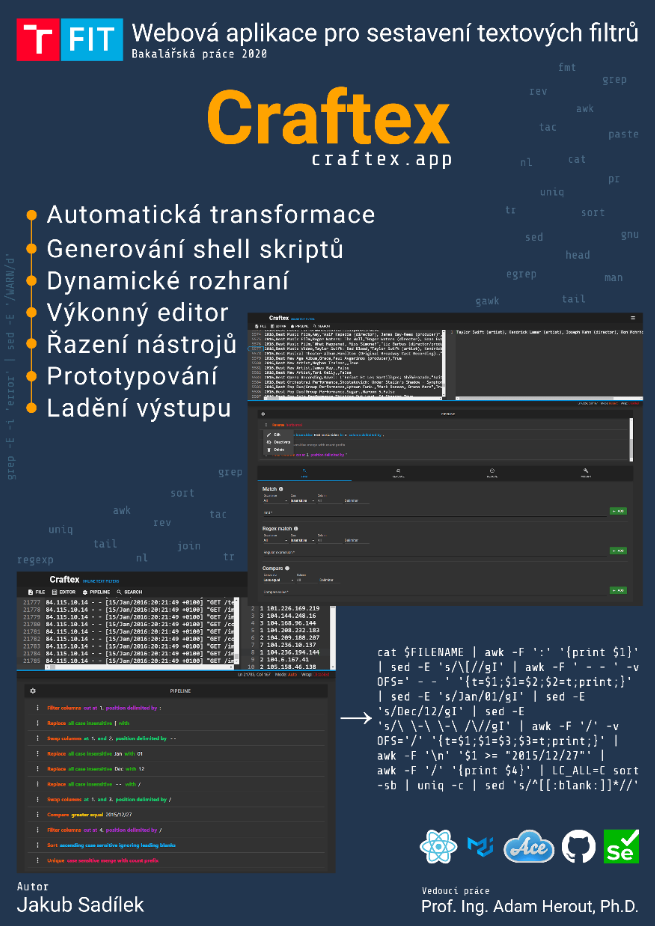
\includegraphics[width=0.71\textwidth]{obrazky-figures/Plakat_zredukovany.PNG}
	\caption{Prezentační plakát webové aplikace ve snížené kvalitě.}
\end{figure}

%=================================================================
\chapter{Obsah přiloženého paměťového média}
V této příloze je popsán obsah přiloženého paměťového média, který je zobrazen na obrázku~\ref{obr:ObsahMedia}.
\begin{figure}[H]
	\centering
	\setlength{\fboxsep}{4pt}
	\fbox{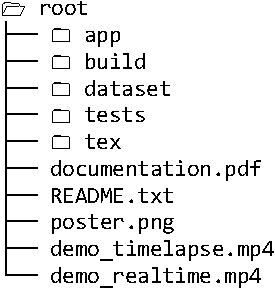
\includegraphics[width=0.25\textwidth]{obrazky-figures/struktura_media.pdf}}
	\caption{Obsah paměťového média.}
	\label{obr:ObsahMedia}
\end{figure}
\begin{itemize}
    \item \textbf{app} -- Adresář obsahuje zdrojové kódy implementované aplikace.
    \item \textbf{build} -- Adresář obsahuje zkompilované zdrojové kódy aplikace pro doménu \url{https://craftex.app}, proto je nelze odtud spustit a jsou zde uvedeny pouze pro úplnost.
    \item \textbf{dataset} -- Adresář obsahuje datovou sadu s případy vhodnými k filtraci.
    \item \textbf{tests} -- Adresář obsahuje zdrojové kódy automatizovaných testů.
    \item \textbf{tex} -- Adresář obsahuje zdrojový tvar technické zprávy.
    \item \textbf{documentation.pdf} -- Technická zpráva.
    \item \textbf{README.txt} -- Manuál obsahující informace k instalaci a obsahu média.
    \item \textbf{poster.png} -- Prezentační plakát aplikace v plné kvalitě.
    \item \textbf{demo\_timelapse.mp4} -- Zrychlené demonstrační video.
    \item \textbf{demo\_realtime.mp4} -- Demonstrační video v reálném čase.
\end{itemize}

%=================================================================
\chapter{Instalační manuál}
V této příloze je popsán postup pro zprovoznění webové aplikace v prostředí Reactu a~implementovaných testů na frameworku Selenium. Proces instalace byl testován na linuxové distribuci Ubuntu 20.04 LTS.

\section{Instalace aplikace}
Následující kroky nainstalují potřebný software stejných verzí, které byly použity při implementaci, přestože mohou fungovat i jiné. Aplikace je také dostupná na webovém portálu \url{https://craftex.app}.

\subsection*{Instalace Node.js verze v12.13.0}
\begin{enumerate}
    \item \texttt{sudo apt-get update}
\end{enumerate}
Pro instalaci specifické verze Node.js je zapotřebí Node Version Manager (NVM).
\begin{enumerate}[resume]
    \item \texttt{sudo apt install curl}
    \item \texttt{curl -o-\newline https://raw.githubusercontent.com/creationix/nvm/v0.33.11/install.sh\newline | bash}
    \item Nyní je nutné zavřít a znovu otevřít terminál, tím bude povoleno NVM.
\end{enumerate}
Kontrola nainstalované verze NVM.
\begin{enumerate}[resume]
    \item \texttt{nvm -{}-version}
\end{enumerate}
Následujícím příkazem bude provedena instalace požadované verze Node.js (v12.13.0).
\begin{enumerate}[resume]
    \item \texttt{nvm install 12.13.0}
\end{enumerate}
Kontrola nainstalované aktuální verze Node.js.
\begin{enumerate}[resume]
    \item \texttt{node -v}

    \textbf{(Poznámka)} V případě používané jiné verze je potřeba provést kontrolu již nainstalovaných verzí a vybrat v12.13.0 následujícími příkazy:
    
    \texttt{nvm ls}
    
    \texttt{nvm use 12.13.0}
\end{enumerate}

\subsection*{Instalace NPM verze 6.12.0}
Po úspěšné instalaci Node.js verze v12.13.0, automaticky by měl být dostupný NPM verze 6.12.0, který je aktuálně vyžadován. Kontrolu nainstalované verze lze provést následujícím příkazem:
\begin{enumerate}
    \item \texttt{npm -v}
 
    \textbf{(Poznámka)} V případě odlišné verze NPM lze provést instalaci požadované verze následujícím příkazem:
		
	\texttt{sudo npm install -g npm@6.12.0}
\end{enumerate}

\subsection*{Instalace aplikace}
Otevřít kořenový adresář aplikace. V přiloženém paměťovém médiu se jedná o adresář \texttt{/app}.
\begin{enumerate}
    \item \texttt{cd app}
\end{enumerate}
Následujícím příkazem proběhne instalace závislostí aplikace.
\begin{enumerate}[resume]
    \item \texttt{npm install}
    
    \textbf{(Poznámka)} Zobrazení zranitelností po instalaci není nutné věnovat pozornost, v~době odevzdání byly v pořádku a přibývají poměrně pravidelně a spousta z nich jich je stále neopravena NPM. V následujícím odkaze si lze zobrazit přehled: \url{https://www.npmjs.com/advisories}.
\end{enumerate}
Spuštění aplikace (může chvíli trvat).
\begin{enumerate}[resume]
    \item \texttt{npm start}
    
    \textbf{(Poznámka)} V případě potíží je nutné použít právo root uživatele (\texttt{sudo npm start}).
\end{enumerate}
Aplikace bude poté dostupná přes webový prohlížeč na adrese \url{http://localhost:3000/}. V~tomto případě kód běžící na dev serveru není optimalizovaný a aplikace může být pomalejší. Pro vygenerování optimalizovaného kódu je potřebné spustit \texttt{npm run build}. Optimalizovaný kód bude poté umístěn v adresáři \texttt{./build}.

\section{Instalace testů}
Otevřít kořenový adresář s testy. V přiloženém paměťovém médiu se jedná o adresář \texttt{/tests}.
\begin{enumerate}
    \item \texttt{cd tests}
\end{enumerate}
Pro běh je potřeba mít nainstalovaný python 3.6 a pip.
\begin{enumerate}[resume]
    \item \texttt{sudo apt-get update}
    \item \texttt{sudo apt-get install python3-pip}
\end{enumerate}
Instalace Selenium a behave.
\begin{enumerate}[resume]
    \item \texttt{pip3 install selenium}
    \item \texttt{pip3 install behave}
    \item \texttt{sudo apt install python3-behave}
\end{enumerate}
Dále je potřeba zprovoznit webdriver pro ovládání prohlížeče (pro Firefox se jedná o GeckoDriver dostupny na: \url{https://github.com/mozilla/geckodriver/releases}), po stáhnutí je nutné ho umístit do adresáře \texttt{/usr/local/bin} a přidat právo pro spuštění (\texttt{chmod +x}), driver použitý při testováni je umístěn v adresáři \texttt{./drivers}, který lze také použít.
\begin{enumerate}[resume]
    \item \texttt{sudo cp drivers/geckodriver /usr/local/bin}
\end{enumerate}
Instalace GNU AWK (pro kompatibilitu s generovanými skripty).
\begin{enumerate}[resume]
    \item \texttt{sudo apt-get update}
    \item \texttt{sudo apt-get install gawk}
\end{enumerate}
Spuštění testů nyní lze provést následujícími příkazy v kořenovém adresáři s testy (\texttt{/tests}).
\begin{itemize}
    \item Spuštění všech testů: \texttt{behave}
    \item Spuštění feature: \texttt{behave -i <název>}
    \item Spuštění scénáře: \texttt{behave -n ``<název>''}
\end{itemize}
